\documentclass{article}
\usepackage{graphicx}
\usepackage{geometry}
\usepackage{hyperref}
\usepackage{mathtools}
\usepackage{float}
\usepackage{minted}
\usepackage{xcolor}
\definecolor{LightGray}{rgb}{0.85,0.85,0.85}
\graphicspath{{./}}
\geometry{a4paper, portrait, margin = 1in}
\title{ROS Made Easy \\1: Workspaces, Packages and Rospy}
\date{\today}
\author{Aniruddh K Budhgavi \\Enigma, IIIT-B}
\begin{document}
    \maketitle
    \section{Important Note}
    This tutorial was created for \textbf{ROS1 Melodic Morenia}
    on \textbf{Ubuntu 18.04 Bionic Beaver}, in \textbf{June 2020}.
    I expect them to become rapidly out of date. It is my hope
    that Team Enigma will continually maintain and update these tutorials.
    \\
    \\
    This tutorial assumes that you are running Ubuntu, and have at least an
    elementary grasp of Python 2.7 and C/C++ .
    \\
    \\
    All the code for this tutorial is available at \url{https://github.com/aniruddhkb/enigmatutorials}.
    \\
    \\
    The aim of this tutorial is to make you \emph{functional} in ROS, not to make you a master. For 
    that, look elsewhere.
    \section{Creating a Catkin workspace}
    \begin{enumerate}
        \item ROS uses a package building system called Catkin. 
        Catkin is built on top of CMake, which 
        enables us to include files from many different directories in a simple way.
        \item Run the following commands
        \begin{minted}[bgcolor=LightGray]{bash}
    :~$ mkdir workspaces 
    :~$ cd workspaces
    :~/workspaces$ mkdir intro2ros
    :~/workspaces/intro2ros$ cd intro2ros
    :~/workspaces/intro2ros$ mkdir src
    :~/workspaces/intro2ros$ catkin_make
        \end{minted}
        You should be fine if the last line of the output is something like:
        \begin{minted}[bgcolor=LightGray]{bash}
    -- Build files have been written to: 
    <path>/intro2ros/workspaces/intro2ros/build
    ####
    #### Running command: "make -j8 -l8" in 
    "<path>/intro2ros/workspaces/intro2ros/build"
    ####    
        \end{minted}
        This sequence of commands:
        \begin{enumerate}
            \item Creates a folder for our workspaces.
            \item Creates a workspace \texttt{intro2ros}
            \item Builds the workspace using the \texttt{catkin\_make} command.
        \end{enumerate}
        \item A \textbf{workspace} is a folder where Catkin packages can be built, modified
         and installed. For some projects, a single workspace is fine, 
         but I like to segment related packages into separate workspaces. Hence the need 
        for a separate folder for them.
        \item The \texttt{catkin\_make} command is used to build all 
        the packages present in that workspace. \textbf{\texttt{catkin\_make} 
        must always be run only from the workspace folder}. The command may fail if there is 
        no \texttt{src} folder in the workspace.
        \item To make sure that ROS recognises packages in your workspace, add the following
        line to your \texttt{.bashrc}:
        \begin{minted}[bgcolor=LightGray]{bash}
    source <path-to-workspace>/intro2ros/devel/setup.bash
        \end{minted}
        Close and restart the terminal.
        Note: If you have mistyped the above command, you may see something like this
        when you reopen the terminal:
        \begin{minted}[bgcolor=LightGray]{bash}
    bash: <path>/intro2ros/devel/setup.bash:
    No such file or directory
        \end{minted}
        \item The source code for the packages in the workspace should be present in the
        \texttt{src} folder of the workspace.
        \item For more information, see \url{http://wiki.ros.org/catkin/workspaces} and
        \url{http://wiki.ros.org/catkin/Tutorials/create_a_workspace}.
    \end{enumerate}
    \section{Creating a package}
    \begin{enumerate}
        \item Run:
        \begin{minted}[bgcolor=LightGray]{bash}
    :~$ roscd
    :.../workspaces/intro2ros/devel$ cd ../src
    :.../workspaces/intro2ros/src$ catkin_create_pkg intro2rospy rospy std_msgs 
            geometry_msgs turtlesim
        \end{minted}
        Output:
        \begin{minted}[bgcolor=LightGray]{bash}
    Created file intro2rospy/CMakeLists.txt
    Created file intro2rospy/package.xml
    Created folder intro2rospy/src
    Successfully created files in <path>/intro2ros/src/intro2rospy.
    Please adjust the values in package.xml.
        \end{minted}
        The \texttt{catkin\_create\_pkg} command is used to create packages
        and \textbf{must be run in the \texttt{src} folder} of your workspace.
        \item To build all the packages in a workspace, run \texttt{catkin\_make}
        from the workspace directory.
        \item Go to the package folder and see what files are there.
        \begin{minted}[bgcolor=LightGray]{bash}
    :.../intro2rospy$ ls
        \end{minted}
        Output:
        \begin{minted}[bgcolor=LightGray]{bash}
    CMakeLists.txt  package.xml  src
        \end{minted}
        \item \texttt{src} is a folder for C++ source files (of which we have none for this package).
        \texttt{package.xml} is a manifest file which tells us and ROS about the package and its dependencies.
        \texttt{CMakeLists.txt} is a configuration file for compilation using CMake.
        \item Let's examine the package manifest. Removing the comments, it looks like:
        \begin{minted}[bgcolor=LightGray]{xml}
    <?xml version="1.0"?>
    <package format="2">
        <name>intro2rospy</name>
        <version>0.0.0</version>
        <description>The intro2rospy package</description>
    
        <maintainer email="akb@todo.todo">akb</maintainer>
    
        <license>TODO</license>
    
        <buildtool_depend>catkin</buildtool_depend>
        <build_depend>geometry_msgs</build_depend>
        <build_depend>rospy</build_depend>
        <build_depend>std_msgs</build_depend>
        <build_depend>turtlesim</build_depend>
        <build_export_depend>geometry_msgs</build_export_depend>
        <build_export_depend>rospy</build_export_depend>
        <build_export_depend>std_msgs</build_export_depend>
        <build_export_depend>turtlesim</build_export_depend>
        <exec_depend>geometry_msgs</exec_depend>
        <exec_depend>rospy</exec_depend>
        <exec_depend>std_msgs</exec_depend>
        <exec_depend>turtlesim</exec_depend>
    
        <export>
    
        </export>
    </package>
        \end{minted}
        \begin{enumerate}
            \item The \texttt{name}, \texttt{version}, \texttt{description}, \texttt{maintainer} 
            and \texttt{license} tags should be obvious.
            \item The \texttt{buildtool\_depend} tag specifies those tools that the package needs
            in order to build itself. Typically, this is only \texttt{catkin}.
            \item The \texttt{build\_depend} tag specifies the packages needed to build this package.
            \item The \texttt{exec\_depend} tag specifies the packages needed to run code in this 
            package.
            \item The \texttt{build\_export\_depend} tag specifies the packages needed for this package to 
            work in a header file for another package. Don't worry if you don't understand this -- it is 
            not relevant for this short course.
            \item The \texttt{export} tag is used for metapackages, which are outside the scope 
            of our discussion.
            Metapackages are packages whose only function is to combine 
            multiple packages which typically work together.
        \end{enumerate}
        \item For more information, see \url{http://wiki.ros.org/catkin/package.xml} and
         \url{http://wiki.ros.org/ROS/Tutorials/CreatingPackage}.
    \end{enumerate}
    \section{Our first ROSPy node}
    \begin{enumerate}
        \item In \texttt{intro2rospy}, create a \texttt{scripts} folder. In this folder,
        create \texttt{hello\_world.py}. The complete file:
        \begin{minted}[bgcolor=LightGray]{python}
    #!/usr/bin/env python
    import rospy
    rospy.init_node('hello_world')
    rospy.loginfo("Hello, world!")
        \end{minted}
        Let's examine it line by line.
        \begin{enumerate}
            \item \mintinline{python}{#!/usr/bin/env python} tells the system that this
            executable should use the Python 2.7 interpreter.
            \item \mintinline{python}{rospy.init_node('hello_world')} creates a new node
            with the name \texttt{hello\_world}.
            \item \mintinline{python}{rospy.loginfo("Hello, world!")} writes a log message,
             which is 
            typically printed to \texttt{STDOUT}.For more information, see 
            \url{http://wiki.ros.org/rospy/Overview/Logging}.
            \item One important point: You cannot define multiple nodes in the
            body of an executable. You can have multiple nodes from the same executable at the
            same time by calling the executable multiple times, 
            but at a time, an executable can spawn only one node.
        \end{enumerate}
        \item Let's edit \texttt{CMakeLists.txt} for \texttt{intro2rospy}.
         Note: This is the \texttt{CMakeLists.txt}
        inside the \texttt{intro2rospy} folder, not the one in the 
        \texttt{intro2ros} folder. Removing the comments, the file is:
        \begin{minted}[bgcolor=LightGray]{cmake}
    cmake_minimum_required(VERSION 3.0.2)
    project(intro2rospy)
    
    find_package(catkin REQUIRED COMPONENTS
        geometry_msgs
        rospy
        std_msgs
        turtlesim
    )
    
    catkin_package()
    
    include_directories(
        include
        ${catkin_INCLUDE_DIRS}
    )
        \end{minted}
        \item Let's examine this line by line.
        \begin{enumerate}
            \item \texttt{cmake\_minimum\_required} and \texttt{project}
            should be obvious.
            \item \texttt{find\_package} is used to specify those CMake packages which 
            we need to build this package.
            \item \texttt{catkin\_package} specifies information specific to Catkin.
            \item \texttt{include\_directories} specifies where the included header files
            can be found. This is relevant to ROSCpp executables we wish to build.
        \end{enumerate}
        \item Add the following to the end of \texttt{CMakeLists.txt}:
        \begin{minted}[bgcolor=LightGray]{cmake}
    catkin_install_python(PROGRAMS
    scripts/hello_world.py
    DESTINATION ${CATKIN_PACKAGE_BIN_DESTINATION}
    )
        \end{minted}
        \texttt{catkin\_install\_python} is used to specify the Python scripts 
        we wish to install.

        \item For more information, see \url{http://wiki.ros.org/catkin/CMakeLists.txt} and 
        \url{http://docs.ros.org/api/catkin/html/howto/format2/installing_python.html}.

        \item Now, run \mintinline{bash}{catkin_make} from the workspace folder. Output:
        \begin{minted}[bgcolor=LightGray]{bash}
    Base path: <path>intro2ros
    Source space: <path>intro2ros/src
    Build space: <path>intro2ros/build
    Devel space: <path>intro2ros/devel
    Install space: <path>intro2ros/install
    ####
    #### Running command: "cmake <path>intro2ros/src 
    -DCATKIN_DEVEL_PREFIX=<path>intro2ros/devel 
    -DCMAKE_INSTALL_PREFIX=<path>intro2ros/install 
    -G Unix Makefiles" in "<path>intro2ros/build"
    ####
    -- Using CATKIN_DEVEL_PREFIX: <path>intro2ros/devel
    -- Using CMAKE_PREFIX_PATH: <path>intro2ros/devel;/opt/ros/melodic
    -- This workspace overlays: <path>intro2ros/devel;/opt/ros/melodic
    -- Found PythonInterp: /usr/bin/python2 (found suitable version "2.7.17"
    , minimum required is "2") 
    -- Using PYTHON_EXECUTABLE: /usr/bin/python2
    -- Using Debian Python package layout
    -- Using empy: /usr/bin/empy
    -- Using CATKIN_ENABLE_TESTING: ON
    -- Call enable_testing()
    -- Using CATKIN_TEST_RESULTS_DIR: <path>intro2ros/build/test_results
    -- Found gtest sources under '/usr/src/googletest': gtests will be built
    -- Found gmock sources under '/usr/src/googletest': gmock will be built
    -- Found PythonInterp: /usr/bin/python2 (found version "2.7.17") 
    -- Using Python nosetests: /usr/bin/nosetests-2.7
    -- catkin 0.7.23
    -- BUILD_SHARED_LIBS is on
    -- BUILD_SHARED_LIBS is on
    -- ~~~~~~~~~~~~~~~~~~~~~~~~~~~~~~~~~~~~~~~~~~~~~~~~~
    -- ~~  traversing 1 packages in topological order:
    -- ~~  - intro2rospy
    -- ~~~~~~~~~~~~~~~~~~~~~~~~~~~~~~~~~~~~~~~~~~~~~~~~~
    -- +++ processing catkin package: 'intro2rospy'
    -- ==> add_subdirectory(intro2rospy)
    -- Configuring done
    -- Generating done
    -- Build files have been written to: <path>intro2ros/build
    ####
    #### Running command: "make -j8 -l8" in "<path>intro2ros/build"
    ####
        \end{minted}
        Ideally, your output should look something like that above. You may see "failed" along
        with some error messages if you've made a mistake in one of the steps. Usually, the 
        error message is descriptive enough to get a hint. If not, Google is your friend.
        \item There is one last step -- navigate to the \texttt{scripts} folder 
        and run:
        \begin{minted}[bgcolor=LightGray]{bash}
    :...scripts$ chmod 777 hello_world.py
        \end{minted}
        \item This gives permission to execute the script as a file.
        \item Now, in two terminals, run:
        \begin{minted}[bgcolor=LightGray]{bash}
    :~$ roscore
    :~$ rosrun intro2rospy hello_world.py
        \end{minted}
        Output:
        \begin{minted}[bgcolor=LightGray]{bash}
    [INFO] [1592385468.996500]: Hello, world! 
        \end{minted}
        Congratulations! You have just written your first ROS node, although it doesn't 
        do very much. Next, let's create a simple publisher node.
    \end{enumerate}
    \newpage
    \section{Publishing to Turtlesim}
    \begin{enumerate}
        \item In \texttt{scripts}, create a new script \texttt{random\_publisher.py}. The file:
        \begin{minted}[bgcolor=LightGray]{python}
    #!/usr/bin/env python
    import rospy
    from geometry_msgs.msg import Twist
    import random
    def random_publisher():
        rospy.init_node('random_publisher', anonymous=True)
        pub = rospy.Publisher('/turtle1/cmd_vel', Twist, queue_size=1000)
        rate = rospy.Rate(2)

        while not rospy.is_shutdown():
            to_publish = Twist()
            to_publish.linear.x =random.uniform(0, 1)
            to_publish.angular.z = random.uniform(-1, 1)
            rospy.loginfo(str(to_publish))
            pub.publish(to_publish)
            rate.sleep()

    if __name__ == "__main__":
        random_publisher()
        \end{minted}
        Let's examine this line-by-line.
        \begin{enumerate}
            \item \mintinline{python}{from geometry_msgs.msg import Twist} -- We need 
            to import the classes for the messages we wish to use.
            \item \mintinline{python}{import random} -- for random number generation.
            \item \mintinline{python}{anonymous=True} -- This ensures that even if 
            we run the same executable multiple times in the same session, the nodes 
            all have unique names. All nodes are uniquely identified by their full name,
            so this is important.
            \item \mintinline{python}{rospy.Publisher('/turtle1/cmd_vel', Twist, queue_size=1000)}
            -- creates a publisher for the topic \texttt{/turtle1/cmd\_vel}, publishing 
            \texttt{geometry\_msgs/Twist} messages, with a queue size of 1000. Basically, if the 
            messages are generated faster than the publisher can publish them, then the publisher
            must store the messages in a queue. The size of this queue is specified here. If more 
            messages are waiting than the queue size, the new messages which are causing the queue
            to overflow are dropped.
            \item \mintinline{python}{rate = rospy.Rate(2)} sets up a rate object of 2 Hertz. We'll
            see more about this in a moment.
            \item \mintinline{python}{rospy.is_shutdown()} checks whether the node has received a 
            shutdown request.
            \item The next section,
            \begin{minted}{python}
    to_publish = Twist()
    to_publish.linear.x =random.uniform(0, 1)
    to_publish.angular.z = random.uniform(-1, 1)
            \end{minted}
            Creates a \texttt{geometry\_msgs/Twist} message and sets the linear and angular parts
            accordingly. The linear part is given a random number between 0 and 1, and the angular
            between -1 and 1.
            \item \mintinline{python}{pub.publish(to_publish)} publishes the message.
            \item \mintinline{python}{rate.sleep()} is used to enforce the frequency at which we
            wish to publish the messages. It measures the time taken by the other parts of the 
            loop and pauses execution such that the rate of message publishing matches the 
            frequency we passed to the rate object earlier.
            \item \mintinline{python}{if __name__ == "__main__":} -- if we are directly executing
            this file and not importing it elsewhere, run the function.
        \end{enumerate}
        \item Make the following change to the \texttt{CMakeLists.txt}:
        \begin{minted}[bgcolor=LightGray]{cmake}
    catkin_install_python(PROGRAMS
        scripts/hello_world.py
        scriptS/random_publisher.py
        DESTINATION ${CATKIN_PACKAGE_BIN_DESTINATION}
    )
        \end{minted}
        \item Don't forget to do the \texttt{chmod} step, and run \texttt{catkin\_make}.
        \item Now, in three terminals, run:
        \begin{minted}[bgcolor=LightGray]{bash}
    :~$ roscore
    :~$ rosrun turtlesim turtlesim_node 
    :~$ rosrun intro2rospy random_publisher.py
        \end{minted}
        \item You should see the turtle move with a random velocity. Like this:
        \begin{figure}[H]
            \center
            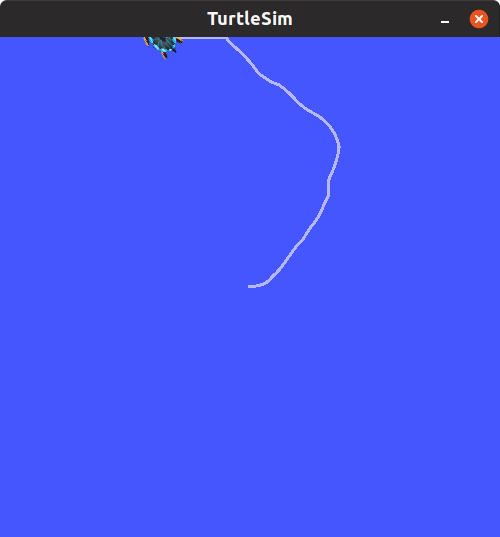
\includegraphics[width = 0.3\textwidth]{turtle.png}
        \end{figure}
        Next, let's write a subscriber node.
    \end{enumerate}
    \newpage
    \section{Subscribing to turtlesim}
    \begin{enumerate}
        \item The subscriber program, \texttt{pose\_subscriber.py} is:
        \begin{minted}[bgcolor=LightGray]{python}
    #!/usr/bin/env python
    import rospy 
    from turtlesim.msg import Pose

    def callback(msg):
        rospy.loginfo(str(rospy.get_name()) + " heard " + str(msg)) 

    def pose_subscriber():
        rospy.init_node("pose_subscriber", anonymous=True)
        rospy.Subscriber("/turtle1/pose", Pose, callback, queue_size=1000)
        rospy.spin()

    if __name__ == "__main__":
        pose_subscriber()
        \end{minted}
        Let's  break this down line-by-line.
        \begin{enumerate}
            \item \mintinline{python}{rospy.Subscriber("/turtle1/pose", Pose, callback, queue_size=1000)}
            -- this sets up a subscriber to \texttt{/turtle1/pose} with message type 
            \texttt{turtlesim/Pose}, using \texttt{callback}, the function defined above, as 
            the callback function. Whenever the subscriber receives a message on that
            topic, the callback function is executed, with the message being the argument. Lastly,
            we have the queue size. Incoming messages are placed in a queue, and messages can only 
            be processed as fast as the execution of the callback function (among other things).
            \item \mintinline{python}{rospy.spin()} hands over the execution of the program to ROS.
            The execution of the callback can only happen if \mintinline{python}{rospy.spin()} or 
            \mintinline{python}{rospy.spinOnce()} is called. For more information, see 
            \url{http://wiki.ros.org/roscpp/Overview/Callbacks%20and%20Spinning}.
            \item \mintinline{python}{rospy.loginfo(str(rospy.get_name()) + " heard " + str(msg))} -- 
            \texttt{rospy.get\_name()} gives us the full name of the node.
        \end{enumerate}
        \item Make the necessary changes to CMakeLists and the permissions. Now, run:
        \begin{minted}[bgcolor=LightGray]{bash}
    :~$ roscore
    :~$ rosrun turtlesim turtlesim_node 
    :~$ rosrun turtlesim turtle_teleop_key
    :~$ rosrun intro2rospy pose_subscriber.py
        \end{minted}
        Control the turtle and see the change in the pose. Output:
        \begin{minted}[bgcolor=LightGray]{bash}
    ...    
    [INFO] [<time>]: /pose_subscriber_11334_1592393854263 heard 
    x: 7.41065740585
    y: 8.16551113129
    theta: 0.639999985695
    linear_velocity: 0.0
    angular_velocity: 0.0
    ...
        \end{minted}
    \item For more information, see \url{http://wiki.ros.org/ROS/Tutorials/WritingPublisherSubscriber%28python%29}.
    \end{enumerate}
    \section{Looking ahead}
    You have written subscriber and publisher nodes, key features of ROS. With this knowledge,
    you should be able to make many non-trivial programs using ROSPy, though you may not yet be 
    able to control robots using ROS. Next time, we will see how to write subscribers and publishers 
    using ROSCpp.
\end{document}